\chaptercover{Prototypes}{chap:Implementation}
{In this chapter, we present the requirements, design and implementation of the two proposed prototypes, from a broader perspective of the component diagram to a detailed description of the implementation details. Section~\ref{chap:Implementation-OCLHighlightPlugin} concerns the OCL Highlight Plugin, followed by Section~\ref{chap:Implementation-OCLComplexityPlugin}, were OCL Complexity Plugin is described.}

As mentioned in previous sections, in this dissertation we propose a tool-based learning feature, dubbed "OCL Highlight Plugin", and an investigation feature, entitled "OCL Complexity Plugin", reified as plugins to Bremen's USE tool. 
Both plugins make use of the same components provided by USE, as presented in the~\gls{componentDiagram} in Figure~\ref{fig:05_componentdiagram}. The concrete implementation of each plugin is described in detail in the following sections.

To make use of these plugins, users should download the corresponding ~\textit{.jar} files (available in each of the corresponding GitHub~\cite{github} repositories indicated below) and place it in the ~\textit{plugins} folder of USE's installation. After restarting USE, two new buttons will show up: clicking on the red marker icon opens the OCL Highlight Plugin, and the green ruler icon will pop-up the OCL Complexity Plugin window. The user should then proceed to import a ~\textit{.usefile} with the definition of the model and a ~\textit{.soil} file with its instantiation (objects). Creating a Class Diagram view is an additional step to make use of the highlight feature.

\begin{figure*}[ht]
    \centering
    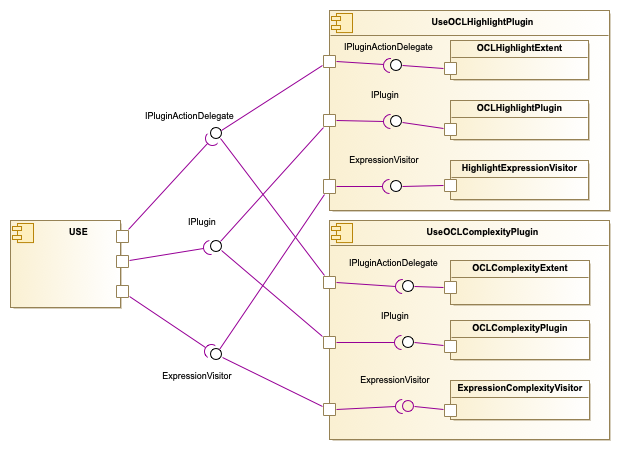
\includegraphics[width=1\textwidth]{Chapters/figures/5_Implementation/ComponentDiagram}
    \caption{OCL Highlight Plugin and OCL Complexity Plugin: Component Diagram}
    \label{fig:05_componentdiagram}
\end{figure*}

\section{OCL Highlight Plugin}
\label{chap:Implementation-OCLHighlightPlugin}

The purpose of the OCL Highlight Plugin is to allow the user to highlight the elements of a UML Class Diagram that are referenced in an OCL expression. These elements include Classes, Attributes, Operations and Relationships. By using strong colours to emphasize the mentioned elements, while painting the rest in lighter colours, we aim to focus the attention of the user on the components that are relevant to the expression under study.

Since USE already includes a coverage option to highlight the elements of the UML Class Diagram that are accessed by each invariant, pre-and post-condition or query operation, the starting point for our work was already in place, speeding up the prototyping phase. The coverage given by USE can be seen in a discriminate way (using the elements browser to select a specific query), or in a integrate way (displaying all the defined queries at the same time). The highlight proposed on this thesis is presented in a dynamic way, whereas in USE  (Gogolla et al.~\cite{GogollaHH14, GogollaHHS15}) it's defined as static (structural coverage when the model is compiled).

\subsection{Requirements}

A set of technical and functional requirements are described for this plugin, not only stating the main functionalities but also some optional yet desired operations that improve its usability. As a technical requirement, it was defined that the plugin should be compatible with USE, meaning that the user can access it's functionalities when working with this tool. In regards to functional requirements, the main use case is that, as a user, I can insert OCL expressions and request the system to highlight it's elements on a Class Diagram. As non-essentials requirements, it was stated that the user could reset the highlighting of the Class Diagram, in order to visualize it as it was initially (default colours defined by USE), and it was suggested that the user could configure the colours of the highlight for each specific element of a Class Diagram (Class, Enum, Attribute, Operation, Rolename and Edge). 
The different use cases defined for this plugin are shown in a Use Case Diagram (Figure~\ref{fig:05_01_usecasediagram}), and typical usage is presented in an Activity Diagram (Figure~\ref{fig:05_01_activitydiagram}).

\begin{figure*}[ht]
    \centering
    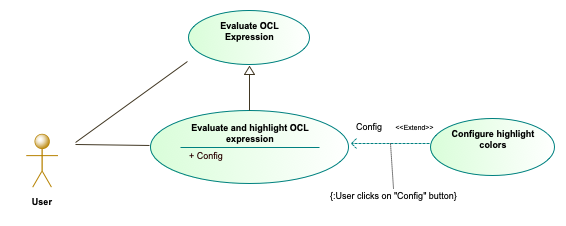
\includegraphics[width=0.9\textwidth]{Chapters/figures/5_Implementation/01_UseCaseDiagram}
    \caption{OCL Highlight Plugin: Use Case Diagram}
    \label{fig:05_01_usecasediagram}
\end{figure*}
    
\begin{figure*}[ht]
    \centering
    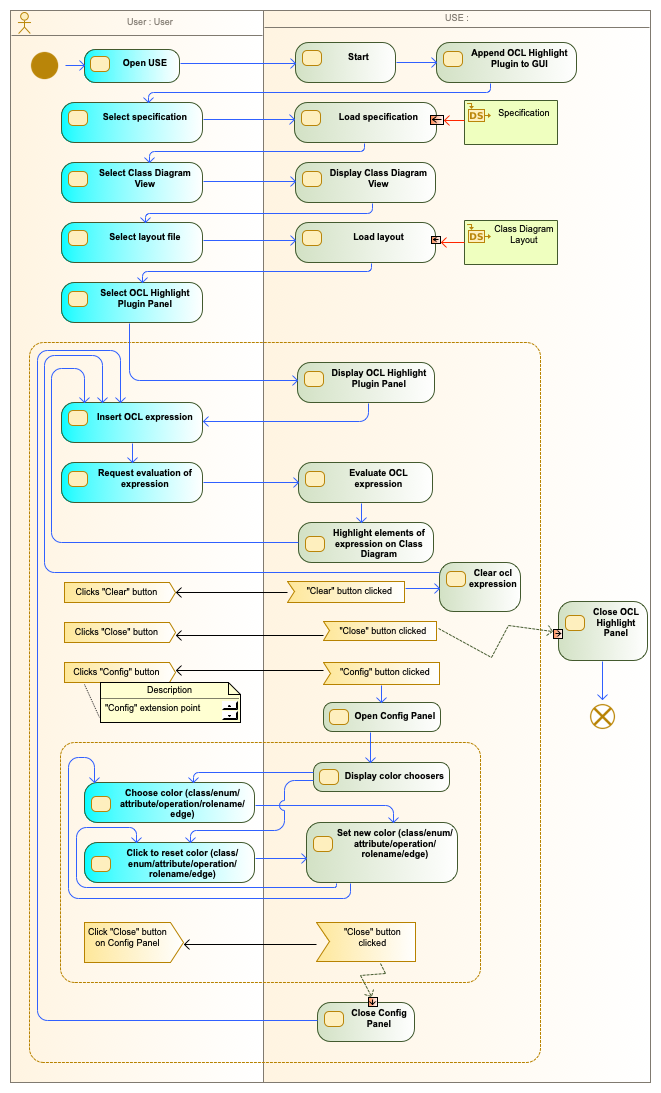
\includegraphics[width=0.9\textwidth]{Chapters/figures/5_Implementation/01_ActivityDiagram}
    \caption{OCL Highlight Plugin: Activity Diagram}
    \label{fig:05_01_activitydiagram}
\end{figure*}

\subsection{Design}

In this subsection, we describe the design of the plugin. Figure~\ref{fig:05_01_classdiagram} presents the Class Diagram, whereas Figure~\ref{fig:05_01_packagediagram} shows the Package Diagram. The implementation of this plugin consisted of the development of the five classes described below: 

\begin{figure*}[ht]
    \centering
    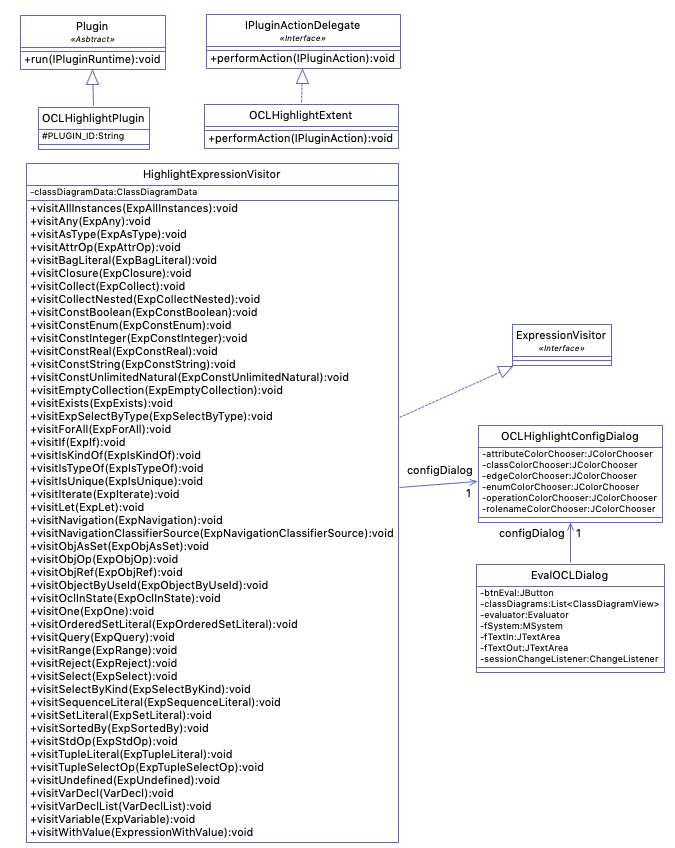
\includegraphics[width=1\textwidth]{Chapters/figures/5_Implementation/01_ClassDiagram}
    \caption{OCL Highlight Plugin: Class Diagram}
    \label{fig:05_01_classdiagram}
\end{figure*}

\begin{figure*}[ht]
    \centering
    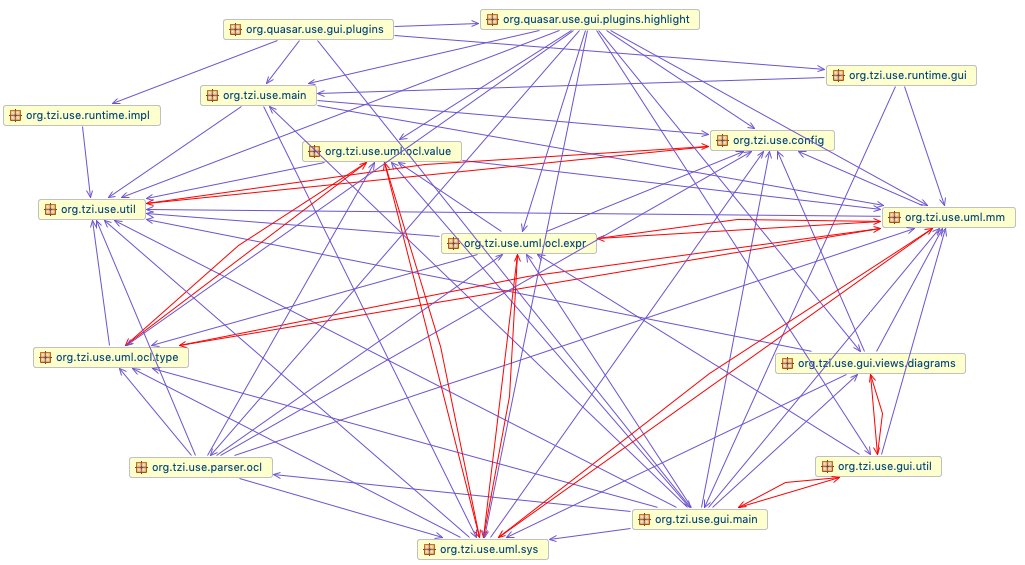
\includegraphics[width=1\textwidth]{Chapters/figures/5_Implementation/01_PackageDiagram}
    \caption{OCL Highlight Plugin: Package Diagram}
    \label{fig:05_01_packagediagram}
\end{figure*}

\textbf{(1) OCLHighlightPlugin:} Main class of the OCL Highlight Plugin. This class defines the id used to identify the plugin. The attribute of this class is shown in Table~\ref{fig:05_01_class1}.

\begin{table}[ht]
\centering
\begin{tabular}{@{}ll@{}}
\toprule
\textbf{Attribute} & \textbf{Description}           \\ \midrule
String PLUGIN\_ID         & Id used to identify the plugin \\ \bottomrule
\end{tabular}
\caption{OCL Highlight Plugin: OCLHighlightPlugin class attributes}
\label{fig:05_01_class1}
\end{table}

\textbf{(2) OCLHighlightExtent:} This is the Plugin Action class. It provides the Action which will be performed if the corresponding Plugin Action Delegate in the application is called. In this case, the Action consists of displaying the panel EvalOCLDialog (with highlight functionality). This class has no attributes.

\textbf{(3) EvalOCLDialog:} This class extends the funcionalities of \textit{JDialog}~\cite{javaxswing}, defining the aspect and actions for entering and evaluating OCL expressions (see Figure~\ref{fig:05_01_panel}), including the creation of text components, labels, and buttons (and their respective action). The attributes of this class are shown in Table~\ref{fig:05_01_class3}. 

\begin{figure*}[ht]
    \centering
    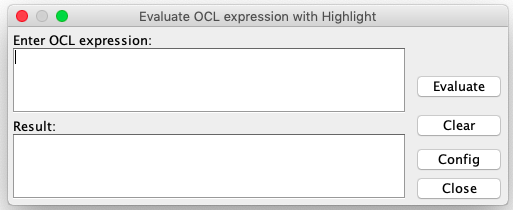
\includegraphics[width=0.8\textwidth]{Chapters/figures/5_Implementation/01_Panel}
    \caption{OCL Highlight Plugin: Panel}
    \label{fig:05_01_panel}
\end{figure*}

\begin{table}[ht]
\centering
\begin{tabular}{@{}ll@{}}
\toprule
\textbf{Attribute}                                         & \textbf{Description}                                                                                                              \\ \midrule
MSystem fSystem                                            & \begin{tabular}[c]{@{}l@{}}Defines the system, including \\ state and functionality\end{tabular}                                  \\ \midrule
JTextArea fTextIn                                          & \begin{tabular}[c]{@{}l@{}}Text area that captures the \\ expression introduced by the user\end{tabular}                          \\ \midrule
JTextArea fTextOut                                         & \begin{tabular}[c]{@{}l@{}}Text area that displays the result \\ of the evaluation of the expression \\ from fTextIn\end{tabular} \\ \midrule
Evaluator evaluator                                        & Evaluates expressions                                                                                                             \\ \midrule
JButton btnEval                                            & Button that triggers the evaluator                                                                                                \\ \midrule
List\textless{}ClassDiagramView\textgreater  classDiagrams & List of the available Class Diagrams                                                                                              \\ \midrule
OCLHighlightConfigDialog configDialog                      & Dialog for configuring highlight colours                                                                                           \\ \midrule
ChangeListener sessionChangeListener                       & \begin{tabular}[c]{@{}l@{}}Change Listener that configures the \\ session of the fSystem\end{tabular}                             \\ \bottomrule
\end{tabular}
\caption{OCL Highlight Plugin: EvalOCLDialog class attributes}
\label{fig:05_01_class3}
\end{table}

\textbf{(4) HighlightExpressionVisitor:} This is the Expression Visitor Class, which implements the methods from the interface \textit{ExpressionVisitor} (available in USE), painting the visited classes of a given OCL expression. The attributes of this class are shown in Table~\ref{fig:05_01_class4}.

\begin{table}[ht]
\centering
\begin{tabular}{@{}ll@{}}
\toprule
\textbf{Attribute}                    & \textbf{Description}                                                                           \\ \midrule
ClassDiagramData classDiagramData     & \begin{tabular}[c]{@{}l@{}}Encapsulates all elements present\\ in a Class Diagram\end{tabular} \\ \midrule
OCLHighlightConfigDialog configDialog & Dialog for configuring highlight colours                                                        \\ \bottomrule
\end{tabular}
\caption{OCL Highlight Plugin: HighlightExpressionVisitor class attributes}
\label{fig:05_01_class4}
\end{table}

\textbf{(5) OCLHighlightConfigDialog:} A dialog for configuring OCL Highlight colours. Similar to EvalOCLDialog, this class extends the funcionalities of \textit{JDialog} (see Figure~\ref{fig:05_01_configcolors}), and defines a set of default colours that can be customized by the user. The attributes of this class are shown in Table~\ref{fig:05_01_class5}.

\begin{figure*}[ht]
    \centering
    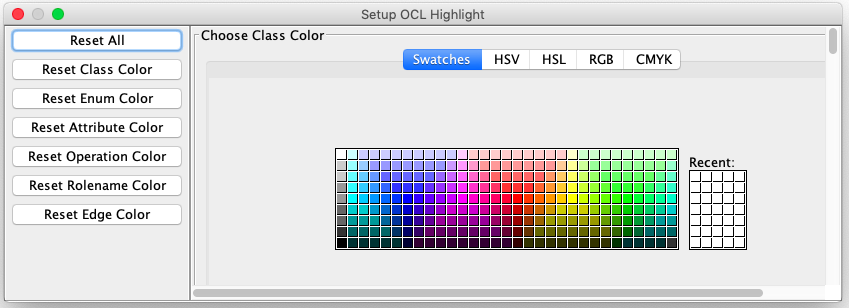
\includegraphics[width=0.8\textwidth]{Chapters/figures/5_Implementation/01_ConfigColors}
    \caption{OCL Highlight Plugin: Highlight colour configuration panel}
    \label{fig:05_01_configcolors}
\end{figure*}

\begin{table}[ht]
\centering
\begin{tabular}{@{}ll@{}}
\toprule
\textbf{Attribute}                                                                                                                                                                           & \textbf{Description}                                                                                                                            \\ \midrule
\begin{tabular}[c]{@{}l@{}}Color CLASS\_COLOR,\\ ENUM\_COLOR,\\ ATTRIBUTE\_COLOR,\\ OPERATION\_COLOR,\\ ROLENAME\_COLOR,\\ EDGE\_COLOR\end{tabular}                                          & \begin{tabular}[c]{@{}l@{}}Default colour for classes, enums,\\ attributes, operations, rolenames, and\\ edge, respectively\end{tabular}  \\ \midrule
\begin{tabular}[c]{@{}l@{}}JColorChooser classColorChooser, \\ enumColorChooser, \\ attributeColorChooser, \\ operationColorChooser,\\ rolenameColorChooser,\\ edgeColorChooser\end{tabular} & \begin{tabular}[c]{@{}l@{}}Colour choosers for classes, enums,\\ attributes, operations, rolenames, and\\ edge, respectively\end{tabular} \\ \bottomrule
\end{tabular}
\caption{OCL Highlight Plugin: OCLHighlightConfigDialog class attributes}
\label{fig:05_01_class5}
\end{table}

\subsection{Implementation}

The OCL Highlight Plugin was developed in Java 8~\cite{java} as an extension for USE. This plugin implements a new OCL evaluation dialog, which resembles the one that is already available in the tool, offering syntax highlighting in the UML Class Diagram when users evaluate a given OCL expression. The OCL expressions are parsed and evaluated using a Visitor pattern~\cite{visitor}, that inherits the functionalities from the interface \textit{ExpressionVisitor} that is made available by USE. After the evaluation, the corresponding UML Diagram elements (such as classes and properties) are highlighted, using a colour that is different to the one provided as default (allowing them to stand out from the rest of the components). Since the API provided by the original tool did not always expose methods and properties to customize the components of the Class Diagram, it was crucial to make the necessary changes using reflection~\cite{reflection}. The concrete implementation of this plugin is available in Github~\cite{useOCLHighlightPlugin}, and a short demo video is accessible in Youtube~\cite{useOCLHighlightPluginDemo}.
 
\subsection{Examples of usage}
\label{chap:Implementation-OCLHighlightPlugin-Examples}

As examples of the behaviour of the plugin, expressions 1 and 2 illustrate the syntax highlighting provided by the evaluation dialog, using the Royal and Loyal model~\cite{Warmer2003}.

\begin{figure*}[ht]
    \centering
    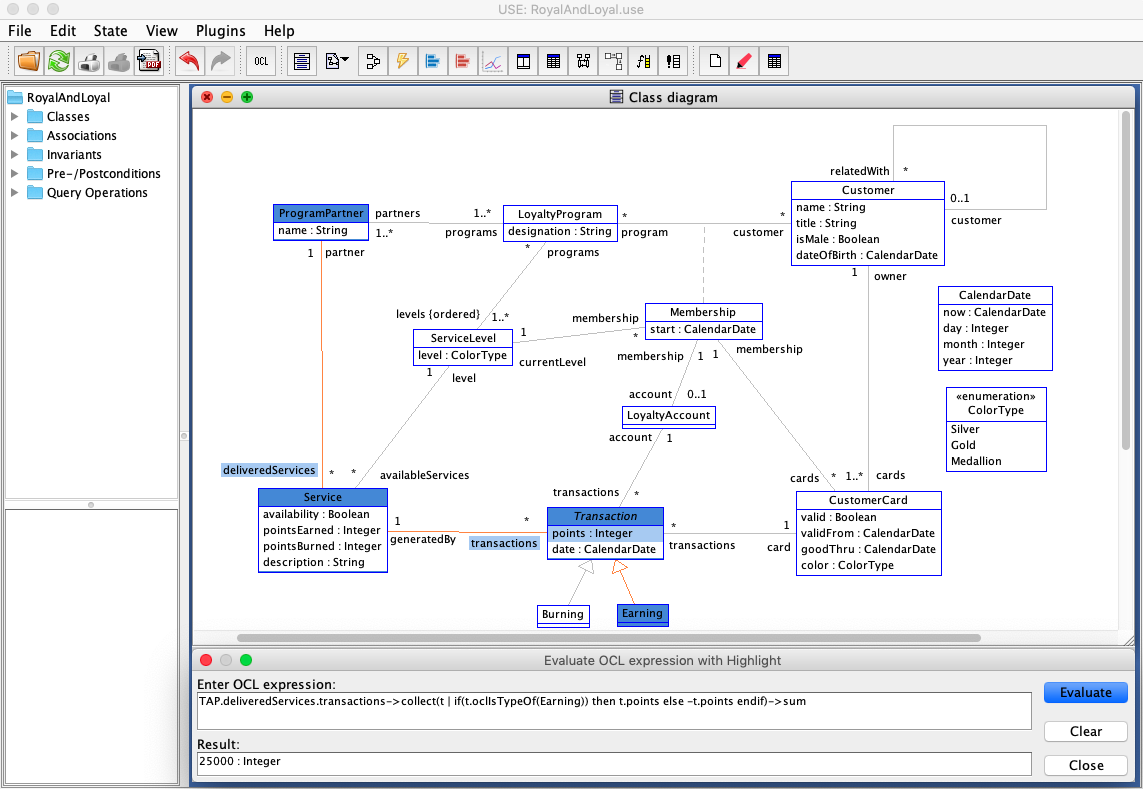
\includegraphics[width=0.94\textwidth]{Chapters/figures/5_Implementation/01_Expression_1}
    \caption{OCL Highlight Plugin: Expression 1}
    \label{fig:01_oclhighlightplugin}
\end{figure*}

\textbf{Expression 1}: This expression exemplifies how to get the balance of points of TAP, which is an instance of \textit{ProgramPartner}. The correspondent highlight is illustrated in Figure~\ref{fig:01_oclhighlightplugin}. The highlighted element are: \textit{ProgramPartner} class, which represents TAP; the navigation from \textit{ProgramPartner} to \textit{Service} (rolename \textit{deliveredServices}), and the \textit{Service} class; and the navigation from \textit{Service} to \textit{Transaction} (rolename \textit{transaction}), and the class \textit{Transaction}. In this expression we want to collect the sum of \textit{points} (property) of a \textit{Transaction}. If a \textit{Transaction} is of type \textit{Earning}, the points are counted positively. If not, they are counted negatively. Both \textit{Earning} and \textit{points} of \textit{Transaction} are also highlighted.

\begin{lstlisting}[caption={OCL expression 1}\label{lst:ocl_expression_1}]
TAP.deliveredServices.transactions
    ->collect(t | if(t.oclIsTypeOf(Earning)) 
        then t.points else - t.points endif)
    ->sum
\end{lstlisting}

\begin{figure*}[ht]
    \centering
    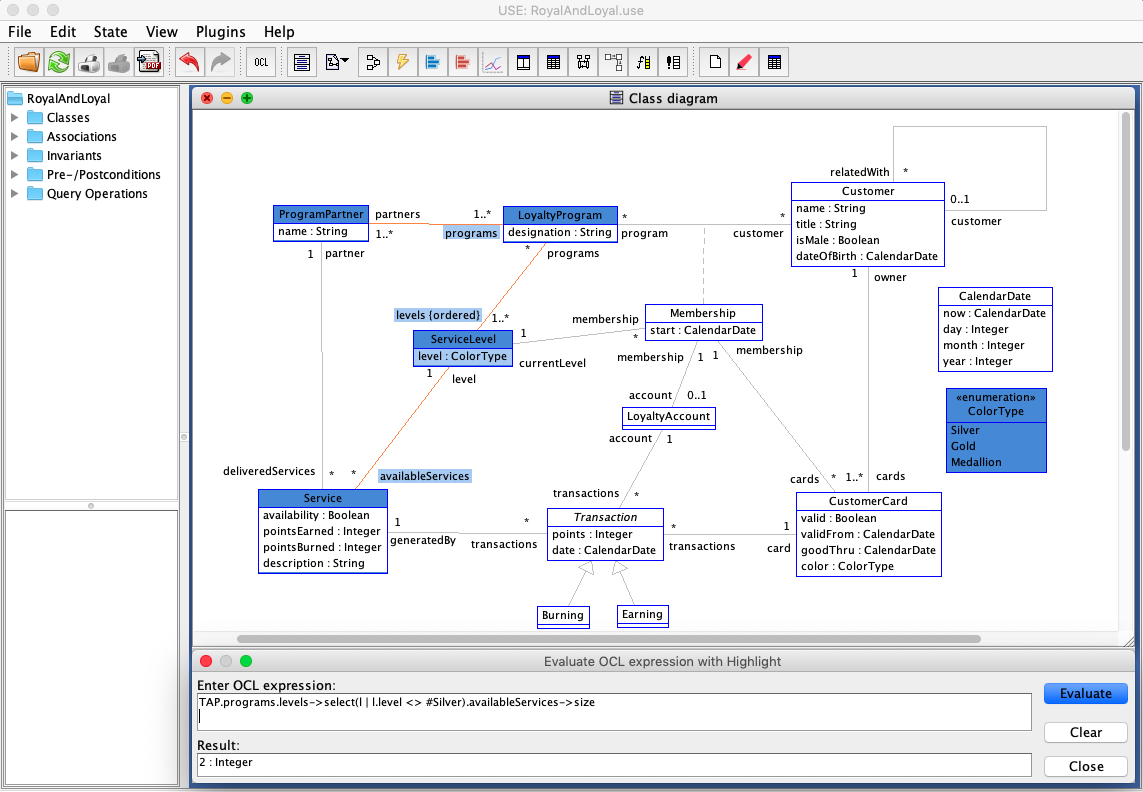
\includegraphics[width=0.94\textwidth]{Chapters/figures/5_Implementation/01_Expression_2}
    \caption{OCL Highlight Plugin: Expression 2}
    \label{fig:02_oclhighlightplugin}
\end{figure*}

\textbf{Expression 2}: This expression exemplifies how to get the number of non-Silver services provided by TAP in the participating Loyalty Programs. The correspondent highlight is illustrated in Figure~\ref{fig:02_oclhighlightplugin}. The highlighted elements are: \textit{ProgramParner}, which again represents TAP; the navigation between \textit{ProgramPartner} and \textit{LoyaltyProgram} (rolename \textit{programs}), and \textit{LoyaltyProgram} class; the navigation between \textit{LoyaltyProgram} and \textit{ServiceLevel} (rolename \textit{levels}), and the class \textit{ServiceLevel}; the \textit{level} (property) of the class \textit{ServiceLevel} and its corresponding type (\textit{ColorType} enum); the navigation from \textit{ServiceLevel} to \textit{Service} (rolename \textit{availableServices}), and the class \textit{Service}.

\begin{lstlisting}[caption={OCL expression 2}\label{lst:ocl_expression_2}]
TAP.programs.levels
    ->select(l | l.level <> #Silver)
    .availableServices->size
\end{lstlisting}

\section{OCL Complexity Plugin}
\label{chap:Implementation-OCLComplexityPlugin}

The second and last plugin presented in this thesis is the OCL Complexity Plugin. As our investigation required to study and analyze several OCL complexity metrics (described in Section~\ref{sec:RelatedWork-Metrics}), we decided to provide them as a plugin, to allow users to evaluate the complexity of the expressions in an automated manner. 

\subsection{Requirements}

This plugin shares the technical requirement with the previous one, meaning that it should be compatible with USE. Regarding functional requirements, we defined that the user should be able to insert OCL expressions and request the computation and display of the complexity of the given expression. To improve the usability, we stated that it should be possible to clear the given expression, allowing the user to easily insert a new one. Additionally, we defined that there should be a panel with a brief explanation of each of the metrics that are displayed, to help the user understand the results of the computation. The different use cases defined for this plugin are shown in a Use Case Diagram (Figure~\ref{fig:05_02_usecasediagram}), and a typical usage is presented in an Activity Diagram (Figure~\ref{fig:05_02_activitydiagram}).

\begin{figure*}[ht]
    \centering
    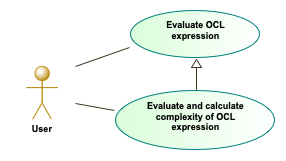
\includegraphics[width=0.6\textwidth]{Chapters/figures/5_Implementation/02_UseCaseDiagram}
    \caption{OCL Complexity Plugin: Use Case Diagram}
    \label{fig:05_02_usecasediagram}
\end{figure*}
  
\begin{figure*}[ht]
    \centering
    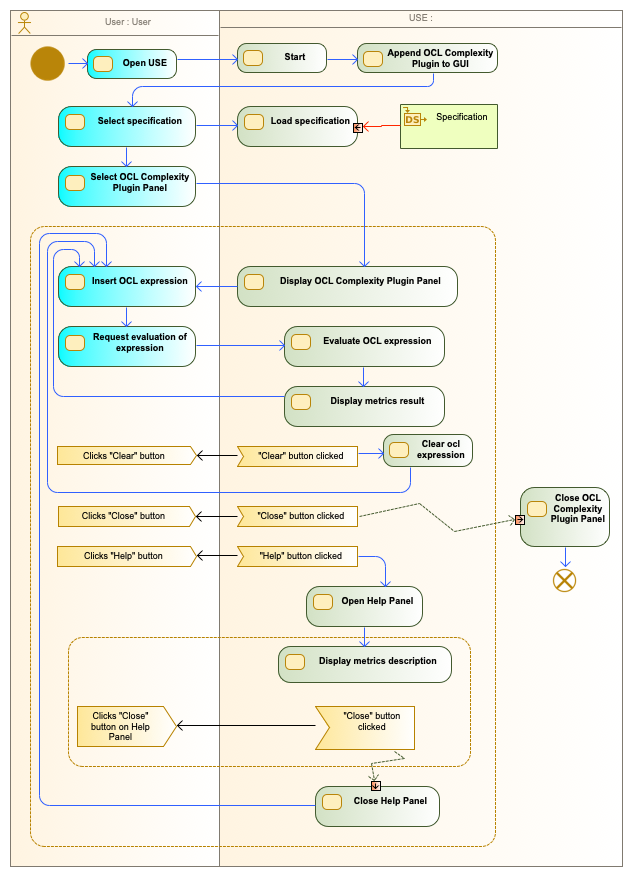
\includegraphics[width=1\textwidth]{Chapters/figures/5_Implementation/02_ActivityDiagram}
    \caption{OCL Complexity Plugin: Activity Diagram}
    \label{fig:05_02_activitydiagram}
\end{figure*}

\subsection{Design}

In this subsection, we describe the design of the plugin. Figure~\ref{fig:05_02_classdiagram} presents the Class Diagram of the implemented system, whereas Figure~\ref{fig:05_02_packagediagram} shows the Package Diagram. The implementation of this plugin consisted of the development of the eight classes and two interfaces described below: 

\begin{figure*}[ht]
    \centering
    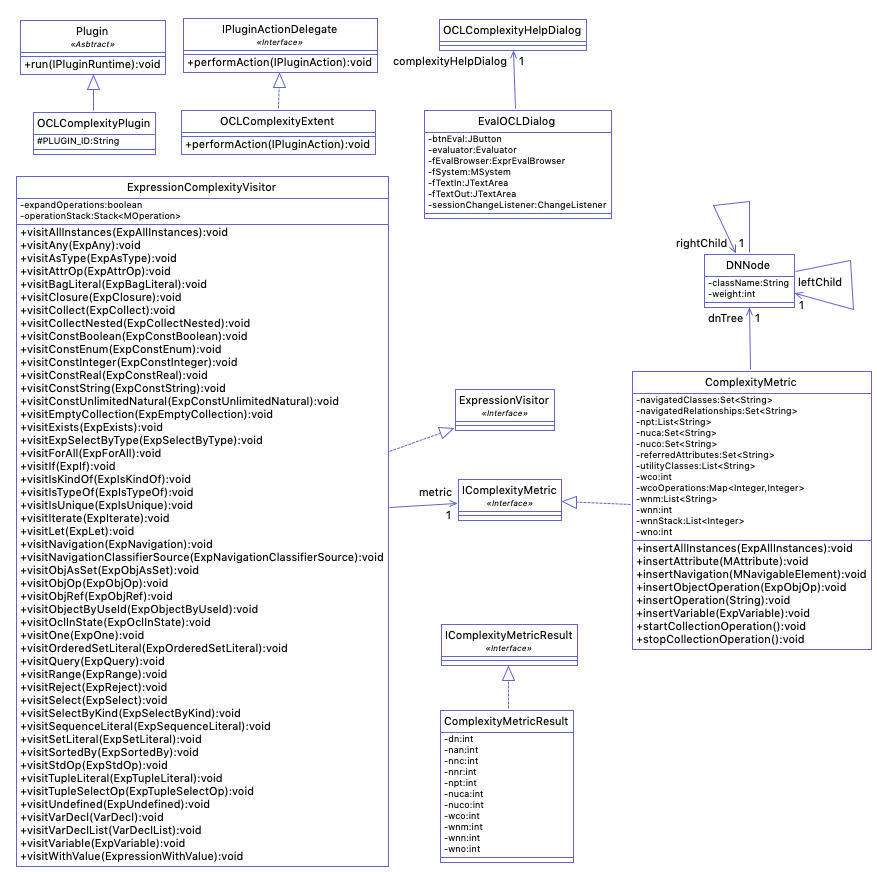
\includegraphics[width=1\textwidth]{Chapters/figures/5_Implementation/02_ClassDiagram}
    \caption{OCL Complexity Plugin: Class Diagram}
    \label{fig:05_02_classdiagram}
\end{figure*}

\begin{figure*}[ht]
    \centering
    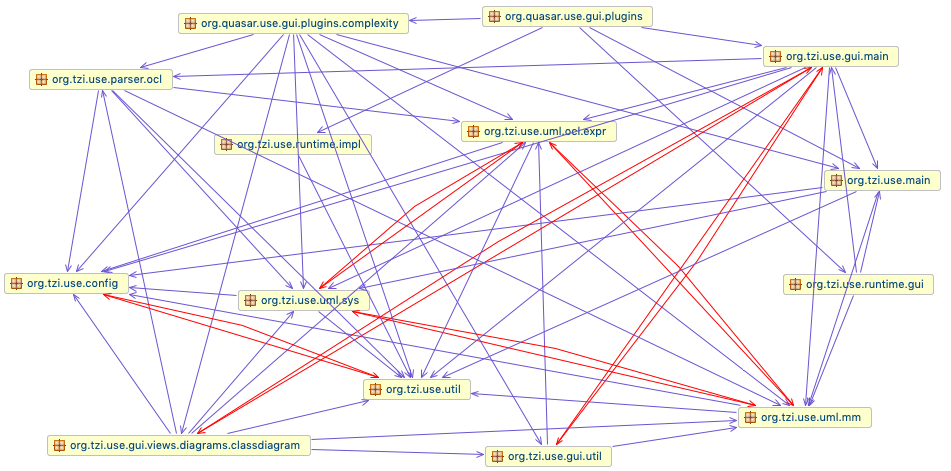
\includegraphics[width=1\textwidth]{Chapters/figures/5_Implementation/02_PackageDiagram}
    \caption{OCL Complexity Plugin: Package Diagram}
    \label{fig:05_02_packagediagram}
\end{figure*}

\textbf{(1) OCLComplexityPlugin:} Main class of the OCL Complexity Plugin. This class defines the id used to identify the plugin. The attribute of this class is shown in Table~\ref{fig:05_02_class1}.

\begin{table}[ht]
\centering
\begin{tabular}{@{}ll@{}}
\toprule
\textbf{Attribute} & \textbf{Description}           \\ \midrule
String PLUGIN\_ID         & Id used to identify the plugin \\ \bottomrule
\end{tabular}
\caption{OCL Complexity Plugin: OCLComplexityPlugin class attributes}
\label{fig:05_02_class1}
\end{table}

\textbf{(2) OCLComplexityExtent:} This is the Plugin Action class. It provides the Action which will be performed if the corresponding Plugin Action Delegate in the application is called. In this case, the Action consists of displaying the panel (with the calculate complexity functionality). This class has no attributes.

\textbf{(3) EvalOCLDialog:} This class extends the funcionalities of \textit{JDialog}~\cite{javaxswing}, defining the aspect and actions for entering and evaluating OCL expressions (see Figure~\ref{fig:05_02_panel}), including the creation of text components, labels, and buttons (and their respective action). The attributes of this class are shown in Table~\ref{fig:05_02_class3}. 

\begin{figure*}[ht]
    \centering
    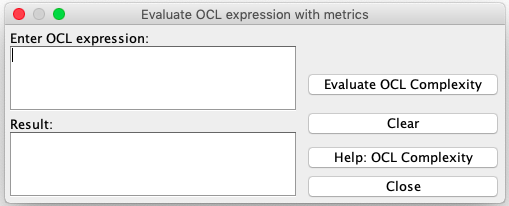
\includegraphics[width=0.8\textwidth]{Chapters/figures/5_Implementation/02_Panel}
    \caption{OCL Complexity Plugin: Panel}
    \label{fig:05_02_panel}
\end{figure*}

\begin{table}[ht]
\centering
\begin{tabular}{@{}ll@{}}
\toprule
\textbf{Attribute}                                        & \textbf{Description}                                                                                                            \\ \midrule
MSystem fSystem                                           & \begin{tabular}[c]{@{}l@{}}Defines the system, including\\ state and functionality\end{tabular}                                 \\ \midrule
JTextArea fTextIn                                         & \begin{tabular}[c]{@{}l@{}}Text area that captures the\\ expression introduced by the user\end{tabular}                         \\ \midrule
JTextArea fTextOut                                        & \begin{tabular}[c]{@{}l@{}}Text area that displays the result\\ of the evaluation of the expression\\ from fTextIn\end{tabular} \\ \midrule
JButton btnEval                                           & \begin{tabular}[c]{@{}l@{}}Button that triggers the complexity \\ evaluation\end{tabular}                                       \\ \midrule
List\textless{}ClassDiagramView\textgreater classDiagrams & List of the available Class Diagrams                                                                                            \\ \midrule
OCLComplexityHelpDialog complexityHelpDialog              & \begin{tabular}[c]{@{}l@{}}Dialog showing an explanation of \\ each complexity metric\end{tabular}                              \\ \midrule
ChangeListener sessionChangeListener                      & \begin{tabular}[c]{@{}l@{}}Change Listener that configures the\\ session of the fSystem\end{tabular}                            \\ \bottomrule
\end{tabular}
\caption{OCL Complexity Plugin: EvalOCLDialog class attributes}
\label{fig:05_02_class3}
\end{table}

\textbf{(4) ExpressionComplexityVisitor:} This is the Expression Visitor Class, which implements the methods from the interface \textit{ExpressionVisitor} (available in USE), calculating the complexity of the expression. The attributes of this class are shown in table~\ref{fig:05_02_class4}. 

\begin{table}[ht]
\centering
\begin{tabular}{@{}ll@{}}
\toprule
\textbf{Attribute}                                    & \textbf{Description}                                                                                         \\ \midrule
Stack\textless{}MOperation\textgreater operationStack & \begin{tabular}[c]{@{}l@{}}Operation stack that controls the navigation\\ on nested operations.\end{tabular} \\ \midrule
IComplexityMetric metric                              & Processes the calculation of metrics.                                                                        \\ \bottomrule
\end{tabular}
\caption{OCL Complexity Plugin: ExpressionComplexityVisitor class attributes}
\label{fig:05_02_class4}
\end{table}

\textbf{(5) ComplexityMetric:} This class calculates and stores the result of the different complexity metrics for an expression. The methods of this class are provided by the interface \textit{IComplexityMetric}, and the attributes are shown in table~\ref{fig:05_02_class5}. 

\begin{table}[ht]
\centering
\begin{tabular}{@{}ll@{}}
\toprule
\textbf{Attribute}                                       & \textbf{Description}                                                                                                              \\ \midrule
Set\textless{}String\textgreater navigatedRelationships  & Set of the navigated relationship names                                                                                           \\ \midrule
Set\textless{}String\textgreater referredAttributes      & Set of the referenced attribute names                                                                                             \\ \midrule
int wno                                                  & Total value of the metric WNO                                                                                                     \\ \midrule
Set\textless{}String\textgreater navigatedClasses        & Set of the navigated classes names                                                                                                \\ \midrule
List\textless{}String\textgreater utilityClasses         & \begin{tabular}[c]{@{}l@{}}List of available utility classes (we \\ only considered "CalendarDate" and \\ "Instant")\end{tabular} \\ \midrule
Set\textless{}String\textgreater nuca                    & \begin{tabular}[c]{@{}l@{}}Set of referenced utility class attribute \\ names\end{tabular}                                        \\ \midrule
Set\textless{}String\textgreater nuco                    & \begin{tabular}[c]{@{}l@{}}Set of referenced utility class operation \\ names\end{tabular}                                        \\ \midrule
int wnn                                                  & Total value of the metric WNN                                                                                                     \\ \midrule
List\textless{}Integer\textgreater wnnStack              & \begin{tabular}[c]{@{}l@{}}Stack of number of operations per depth \\ (on the navigation tree)\end{tabular}                       \\ \midrule
DNNode dnTree                                            & Root of navigation tree                                                                                                           \\ \midrule
Map\textless{}Integer, Integer\textgreater wcoOperations & \begin{tabular}[c]{@{}l@{}}Map of the total of collection operations \\ per depth (on the navigation tree)\end{tabular}           \\ \midrule
int wco                                                  & Total value of the metric WCO                                                                                                     \\ \bottomrule
\end{tabular}
\caption{OCL Complexity Plugin: ComplexityMetric class attributes}
\label{fig:05_02_class5}
\end{table}

\textbf{(6) DNNode:} This class represents a node in the navigation tree. The attributes of this class are shown in table~\ref{fig:05_02_class6}. 

\begin{table}[ht]
\centering
\begin{tabular}{@{}ll@{}}
\toprule
\textbf{Attribute} & \textbf{Description}                      \\ \midrule
String className   & Name of the class represented by the node \\ \midrule
int weight         & Node's weight                             \\ \midrule
DNNode leftChild   & Node's left child                         \\ \midrule
DNNode rightChild  & Node's right child                        \\ \bottomrule
\end{tabular}
\caption{OCL Complexity Plugin: DNNode class attributes}
\label{fig:05_02_class6}
\end{table}

\textbf{(7) ComplexityMetricResult:} This class encapsulates the result of the different complexity metrics for an expression. The methods of this class are provided by the interface \textit{IComplexityMetricResult}, and the attributes are shown in table~\ref{fig:05_02_class7}. 

\begin{table}[ht]
\centering
\begin{tabular}{@{}ll@{}}
\toprule
\textbf{Attribute}                                                                         & \textbf{Description} \\ \midrule
\begin{tabular}[c]{@{}l@{}}int nnr, nan, wno, nnc,\\ nuca, nuco, wnn, dn, wco\end{tabular} & Value of each metric \\ \bottomrule
\end{tabular}
\caption{OCL Complexity Plugin: ComplexityMetricResult class attributes}
\label{fig:05_02_class7}
\end{table}

\textbf{(8) OCLComplexityHelpDialog:} A dialog that displays a short description of each metric. This class extends the functionalities of \textit{JDialog}, with no additional attributes.

\subsection{Implementation}

Similarly to what was described for the OCL Highlight Plugin, this one was also developed in Java 8 as an extension for USE. In this case, the decision to built it for USE instead of another tool was purely based on the fact that, after the development of the first plugin, we already had the knowledge and experience to build an extra functionality for it. The plugins share a similar logic underneath, meaning that they both provide a new evaluation dialog that parses and evaluates expressions using a Visitor pattern. Instead of showing the syntax highlight, this one calculates the complexity metrics of the given expression. The concrete implementation of this plugin is available in Github~\cite{useOCLComplexityPlugin}. In this iteration of the plugin, we decided to exclude the metric WNM, as our models didn't include Messages, and NPT since it's mainly used for pre-and post-conditions, which wasn't part of the questionnaires.

\subsection{Examples of usage}

As examples of the behavior of the plugin, Figure~\ref{fig:02_expression_1} shows the complexity values for Expression~\ref{lst:ocl_expression_1}, whereas Figure~\ref{fig:02_expression_2} presents the values for Expression~\ref{lst:ocl_expression_2} (defined in Subsection~\ref{chap:Implementation-OCLHighlightPlugin-Examples}).

\begin{figure*}[ht]
    \centering
    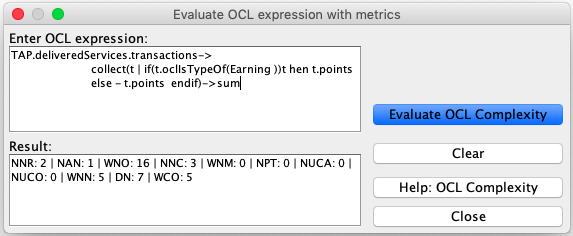
\includegraphics[width=0.8\textwidth]{Chapters/figures/5_Implementation/02_Expression_1}
    \caption{OCL Complexity Plugin: Expression 1}
    \label{fig:02_expression_1}
\end{figure*}

\begin{figure*}[ht]
    \centering
    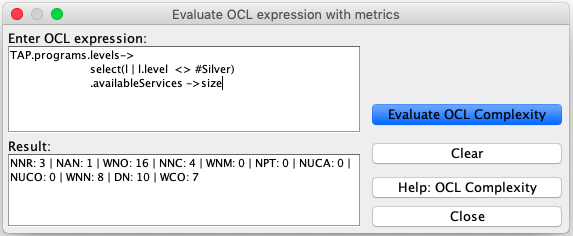
\includegraphics[width=0.8\textwidth]{Chapters/figures/5_Implementation/02_Expression_2}
    \caption{OCL Complexity Plugin: Expression 2}
    \label{fig:02_expression_2}
\end{figure*}


\begin{comment}
1. Requirements
Diagrama de UseCases (descrição em lingua natural com o use case)
- inserir expressao e verificar o highlight
- diagrama de atividades (use cases https://www.modelio.org/)
    duas lanes (utilizador + use)
    
2. Design  
- diagrama de pacotes + diagrama de classes (explicar o que cada classe faz, a sua estrutura, explicar os atributos numa tabela)

3. Implementation
Remeter implementaçao para o github (não é preciso grande descrição)
\end{comment}